% figures/detect/fig_mode_shapes.tex — loads PDF exported from NB03
% Requires \usepackage{graphicx}. Export the PC1 & PC2 loading profiles
% (Sv-scaled: components·√λ, i.e. eof1/eof2) as
% figures/detect/mode_shapes.pdf.
\begin{figure}[!ht]
    \centering
    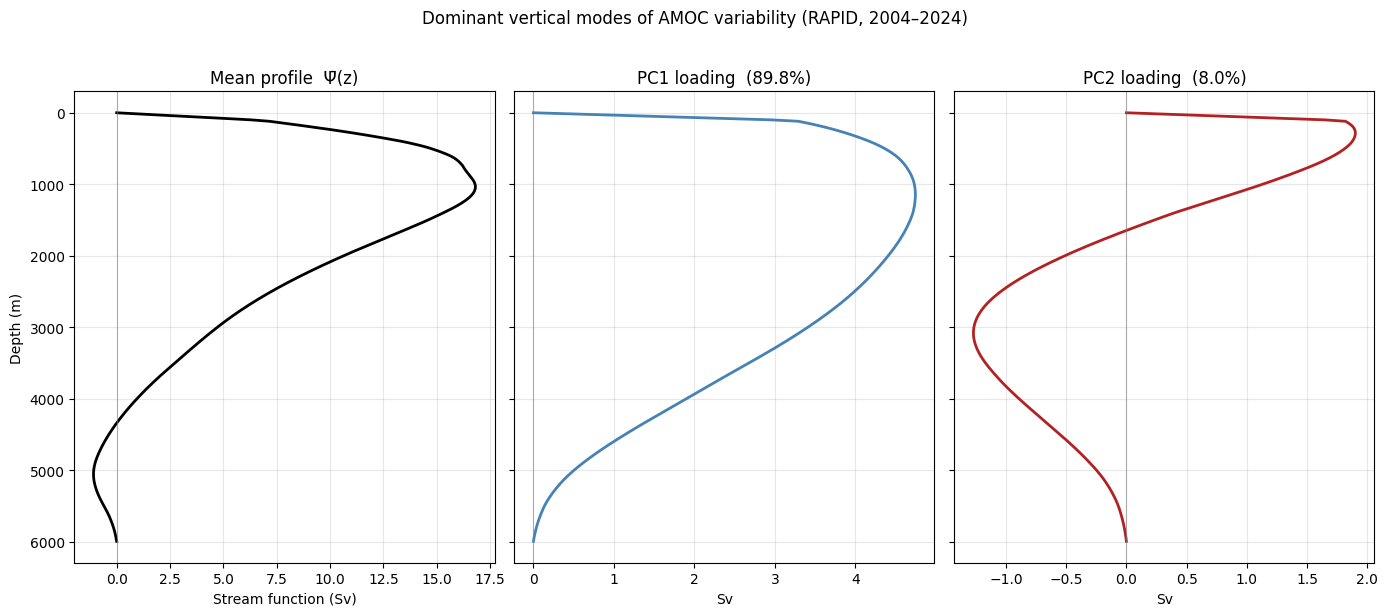
\includegraphics[width=1\textwidth]{figures/data_pipeline/mode_shapes.png}
    \caption[The two vertical modes: intensity and redistribution.]{\textbf{The
    two modes that explain the AMOC's vertical anatomy.} Each curve is a loading
    profile plotted against depth. PC1 (intensity) is a \emph{monopole}: the same
    sign at every depth, peaking near 1150~m where the mean profile peaks, so a
    change in its score strengthens or weakens the whole overturning cell coherently.
    PC2 (redistribution) is a \emph{dipole}: it changes sign once with depth,
    strengthening the cell at one level while weakening it at another. Loadings are
    Sv-scaled for display. Together these two shapes carry \SI{97.86}{\percent} of
    the vertical variability.}
    \label{fig:mode-shapes}
\end{figure}